\pdfoutput=1
\input{glyphtounicode}
\pdfgentounicode=1
\documentclass[conference,10pt,letterpaper]{IEEEtran}
\usepackage[T1]{fontenc}
\usepackage{amsmath,amssymb,booktabs,tabularx,array,graphicx}
\usepackage{cite,url,microtype}
\usepackage[hidelinks]{hyperref}
\graphicspath{{figures/}}
\newcolumntype{Y}{>{\raggedright\arraybackslash}X}
\newcommand{\NC}{C_{\mathrm{NC}}}
\newcommand{\NL}{C_{\mathrm{NL}}}
\newcommand{\Pass}{\textsc{Pass}}
\newcommand{\Fail}{\textsc{Fail}}
\newcommand{\Unk}{\textsc{Indeterminate}}
\setlength{\emergencystretch}{1em}
\title{When Grasp Metrics Disagree:\\Contact, Load, and Retention in Simulation}
\ifdefined\reviewcopy
\author{\IEEEauthorblockN{Anonymous Author}}
\hypersetup{pdfauthor={},pdftitle={When Grasp Metrics Disagree: Contact, Load, and Retention in Simulation}}
\else
\author{\IEEEauthorblockN{Teo Ee Hern}\IEEEauthorblockA{Tianjin University\\eehern27@gmail.com}}
\hypersetup{pdfauthor={Teo Ee Hern},pdftitle={When Grasp Metrics Disagree: Contact, Load, and Retention in Simulation}}
\fi
\begin{document}
\maketitle
\begin{abstract}
A simulated object can touch its environment without receiving load, and can
receive load without depending on it for a specified continuation. Grasp
evaluations that conflate these properties can disagree without either
implementing its stated rule incorrectly. We separate literal no-contact,
realized no-external-load, and intervention-conditioned retention, and test
their consequences using frozen protocols in MuJoCo. Across 240 free-object
controls, no-contact rejects 56 of 77 no-load reference positives; eight
representation-only pairs change its verdict despite identical full-state
trajectories. However, an integrated load-and-geometry monitor provides no
observed gain over a full-wrench baseline on either registered primary
comparison. It rescues none of 85 historical excluded scenes. On 120 fresh
Allegro scenes, both monitors make identical selections or abstentions: 13
returns, 10 successful independent 15-second continuations, and 107 abstentions.
Native-gate selection returns 40 candidates with 15 successful continuations,
exposing a failure-versus-coverage tradeoff rather than uniform improvement.
Fetch and Shadow adapters further reveal task and uncertainty boundaries.
The result is a measurement study with explicit negative findings, not a
superior grasp evaluator: evaluation targets, intervention horizons, and
abstention costs must be stated before acceptance rates can support a claim.
\end{abstract}
\begin{IEEEkeywords}
Grasp evaluation, contact semantics, external load, retention, reproducibility.
\end{IEEEkeywords}

\section{Introduction and Context}
A grasping program lifts an object and holds it near the palm. Has it
succeeded? A native task predicate may accept the motion; a continuous-hold
predicate may reject an interruption; an environment-clear predicate may
reject a contact record even when that record transmits no force. Conversely,
measuring a nonzero environmental load does not establish that the grasp would
fail if that load were removed. These are different questions about the same
robotic execution, not interchangeable degrees of evaluator strictness.

This distinction matters when evaluation is used to select among candidate
grasp schedules. A metric can better match a declared physical target yet
reject useful candidates, or accept a historically unloaded trajectory that
fails during subsequent use. The relevant outcome is then not just the
fraction of returned candidates that work, but also failures and abstentions
per assigned scene. Figure~\ref{fig:targets} grounds the distinction in
free-object controls; the main decision experiment uses a dexterous Allegro
hand and a fixed program library.

\subsection{Relation to Grasp and Execution Evaluation}
Large-scale grasp evaluation supports learned quality prediction and
sim-to-real transfer, as in Get a Grip~\cite{lum2025getagrip}. BODex and
task-oriented wrench estimation address grasp synthesis and mechanical
capacity~\cite{chen2025bodex,chen2023task}; Grasp to Act evaluates dynamic
tool-use requirements~\cite{grasp_to_act2026}. These objectives differ from
identifying loads that actually occurred along a recorded trajectory.
External forces can also be intentionally useful, as established in extrinsic
dexterity~\cite{extrinsic2014}; environmental contact is not intrinsically
an error. SafeManip formalizes temporal safety properties, while Eval-Actions
examines fine-grained execution quality~\cite{huang2026safemanip,eval_actions2026}.
Our focus is narrower: when contact, realized load, and a specified removal
test disagree, what has each measurement established, and does added monitor
complexity improve a frozen selection decision?

\subsection{Contributions and Scope}
We contribute (1) a concrete separation of three evaluation targets, with
full-state paired interventions and independently implemented reconstruction;
(2) a frozen controlled study that establishes a representation-dependent
contact mismatch but finds no incremental benefit of the integrated monitor
over a strong full-wrench baseline; and (3) a sealed candidate-selection study
that makes downstream use and abstention explicit. These contributions concern
measurement validity and bounded negative evidence, not a new grasp planner,
a learned evaluator, or a replacement for reinforcement learning.

Prior custom-hand and open-hand reports~\cite{teo_custom,teo_open} supply
historical development context. The earlier compiled-physics study (V3) is
reported separately in Section~\ref{sec:history}; the frozen measurement study
(V4) supplies the primary comparisons. Their scene sets and evidential roles
remain distinct.

\begin{figure*}[t]
\centering
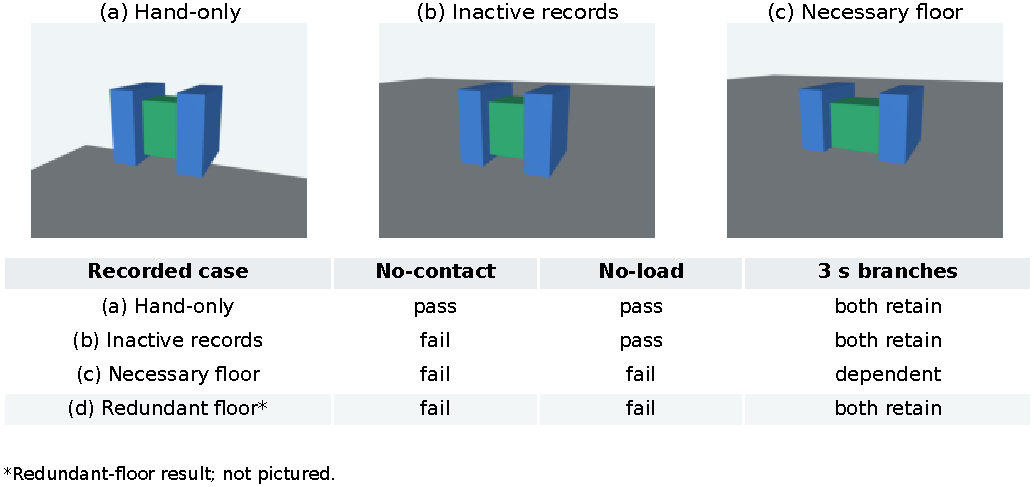
\includegraphics[width=.86\textwidth]{targets.pdf}
\caption{Three existing free-object control renderings, with their recorded
verdicts. The table adds the recorded redundant-floor case: realized loading
and failure after removal are not equivalent. Images illustrate distinct
apparatus cases, not the eight representation-only pairs. A both-retain
outcome is conditional on the specified 3\,s continuation.}
\label{fig:targets}
\end{figure*}

\section{Evaluation Targets}
\subsection{Common Conditions and Literal No-Contact}
For physical step $t$, let $Q_t$ encode source-specific task conditions and
$G$ the unchanged episode-level eligibility rules. Allegro retains native
success, settling and lift boundaries, thumb/opposing-region contact, and
prohibitions on assistance or post-reset target-state edits. Its
$10^{-4}$\,N region-contact floor identifies nonzero contact, not support of
the object's weight. Let $n_t^E$ count target--environment contact records,
including inactive margin records. For continuous interval $I$ and $T=15$\,s,
\begin{equation}
\NC=G\wedge\exists I:\ |I|\ge T,\quad
\forall t\in I,\ Q_t\wedge(n_t^E=0).
\end{equation}
This is a legitimate literal requirement. A rejection is a false negative
only with respect to a \emph{different, explicitly declared} reference target.

\subsection{Realized No-External-Load}
Each environmental contact provides a local force $f_i$, torque $\tau_i$,
frame $R_i$, contact point $p_i$, and sign $s_i$ directing the wrench onto the
target. At target center of mass $c$,
\begin{equation}
F_i=s_iR_i^\top f_i,\qquad
M_i=s_iR_i^\top\tau_i+(p_i-c)\times F_i.
\end{equation}
For object mass $m$ and declared half-diagonal $L$, define
\begin{equation}
r_F=\frac{\sum_{i\in E_t}\|F_i\|+d_F}{mg},\qquad
r_M=\frac{\sum_{i\in E_t}\|M_i\|+d_M}{mgL}.
\label{eq:load}
\end{equation}
The $d_F,d_M$ terms meter known target free-joint damping. Gravity remains
active but is not classified as environmental support. Summing individual
magnitudes prevents opposing loads from canceling into apparent absence.

Both ratios use frozen lower/upper bounds $10^{-4}$ and $10^{-2}$.
A step is definitely unloaded only below both lower bounds with relevant
paths accounted for and ambiguity resolved. Either ratio at or above its
upper bound establishes loading. Intermediate loads, unexplained passive
forces, and unresolved active-zero-load constraints remain unknown.
The geometry guard uses a $10^{-5}$\,m penetration tolerance. Damping is
evaluated at the solve state and implicit endpoint, using the larger magnitude;
unsupported equality, spring, fluid or friction-loss paths cannot silently pass.

Let $I^-$ and $I^+$ be the longest definitely- and possibly-unloaded
continuous $Q$ intervals. Then
\begin{equation}
\NL=\begin{cases}
\Pass,&G\text{ holds and }|I^-|\ge T,\\
\Fail,&G\text{ fails or }|I^+|<T,\\
\Unk,&\text{otherwise.}
\end{cases}
\end{equation}
Telemetry validity is separate: a missing physical step or inconsistent clock
is invalid data, not an observed physical failure. Independent code
reconstructs wrenches, geometry and intervals from saved measurements; it
does not provide independent-engine or hardware ground truth.

\subsection{Intervention-Conditioned Retention}
At fixed $t_0$, two branches start from the complete
\texttt{mjSTATE\_INTEGRATION} state. The sham preserves the model; the removal
branch disables only permitted target--environment contact pairs. Both replay
the same control/mocap tape for $H=3$\,s. Endpoint $Y$ requires displacement
$\le0.03$\,m, rotation $\le0.35$\,rad and speed $\le0.2$\,m/s at every sample,
relative to the initial palm-relative pose (world frame for the pad controls).
The four $(Y_s,Y_e)$ cells are both retain, dependent $(1,0)$, removal rescue
$(0,1)$, and both fail. Dependence therefore means
\begin{equation}
D_{\mathrm{CF}}=1\iff Y_s=1\wedge Y_e=0.
\end{equation}
It is conditional on the chosen state, permitted removal, horizon and open-loop
continuation. It is neither the historical no-load label nor a general
causal statement about grasp ability. The sham must reproduce the original
position/velocity trace bit-for-bit; unreachable or invalid states stay counted.

\begin{figure}[t]
\centering
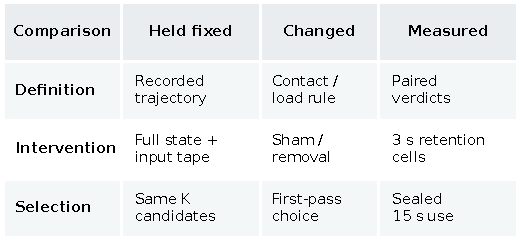
\includegraphics[width=\columnwidth]{contrasts.pdf}
\caption{Three distinct comparisons. Definition contrasts keep the trajectory
fixed; branches change the physical continuation; selection changes the
returned candidate. The separate 15\,s future-use endpoint is evaluated only
after choices are sealed.}
\label{fig:contrasts}
\end{figure}

\section{Frozen Study Design}
\subsection{Evidence Units and Data Roles}
Dynamics use MuJoCo~\cite{todorov2012mujoco}; Allegro derives from
Menagerie~\cite{mujoco_menagerie}. Before final outcomes, an input-only lock
fixed sources, code, seeds, roles, distributions, thresholds, branch timing,
reference sampling, candidate order, analysis and budgets. Eighty development
controls qualified the observer with identical complete integration traces
enabled/disabled; 89 qualification tests passed. Source-specific shams and
observer checks were recorded separately. One implementer operated the
workflow: timestamps and hashes are not independent blinding.

Table~\ref{tab:design} lists final units. The controls use a free six-DOF
target between actuated pads, without a target guide or hidden stabilizer.
Their eight groups are hand-only, inactive-margin, necessary-floor,
redundant-floor, opposed-contact, intermittent-floor, applied-assistance and
boundary-clearance cases (30 each). Half the intermittent group has a single
0.1\,s support burst; half has periodic support. Geometry, mass, friction and
initial perturbations vary within locked ranges. Eight inactive-margin cases
have a margin/gap-only partner; paired invariance is asserted only after full
integration-state equality, not visual similarity.

\begin{table}[t]
\caption{Final units and fixed subsets. Reference and branch samples are
subsets, not additional independent scenes.}
\label{tab:design}\centering\footnotesize
\setlength{\tabcolsep}{3pt}
\begin{tabularx}{\columnwidth}{l r Y}
\toprule
Source & Units & Task; branch / reference subset\\
\midrule
Pad controls & 240 & 18\,s retention; 48 at 8\,s / all 240\\
Allegro & 120 & Six families, 720 schedules; 20 rank-1 states / 30 rank-1 records\\
Fetch expert & 100 & Native 50 actions; separate 500-action retention; 20 / 30\\
Shadow / DGB & 100 & Four object identities; added gravity retention; 20 / 30\\
\bottomrule
\end{tabularx}
\end{table}

The historical development retrospective covers every candidate slot in 85
V3 scenes accepted natively but not by no-contact. Of 510 slots, 177 qualifying
traces received full-wrench replay; 333 already failed common conditions.
Their unmeasured load histories are not imputed. This retrospective is not a
fresh final test.

\subsection{Comparators and External Boundaries}
We use semantic names with frozen identifiers. Native (B0) is the original
Allegro gate; on added control/external tasks it is an accumulated-$Q$ proxy,
not the upstream task score. Continuous (B1) requires contiguous $Q$;
no-contact (B2) is $\NC$; clearance (B3) adds positive geometric clearance.
The primary full-wrench baseline (B4) uses the same force/torque thresholds,
continuous time, passive-load accounting and uncertainty treatment as the
integrated monitor (B5), but omits its geometry guard. B4 is not a weakened
normal-force baseline. Normal-only (B4-normal) is reported separately.

Static feasibility (B6) uses an eight-ray friction cone and bounded actuator
force balance; unsupported actuation is not applicable. A signed-force probe
(B7) applies six one-weight world-axis forces for 1\,s each. These measure
capacity or perturbed future behavior, not historical no-load truth. They use
the fixed branch subset and charge extra steps. Five no-load ablations remove
geometry, torque, per-contact aggregation, uncertainty or continuous time;
five control operating points were fixed before final outcomes.

Fetch uses the public scripted expert~\cite{fetch_expert} with its native
Gymnasium-Robotics goal/reset~\cite{gymnasium_robotics}; table-level goals are
not raised. The added lift/two-finger-contact task retains target damping.
Shadow/DexGraspBench (DGB)~\cite{dexgraspbench} begins from upstream
pregrasp/grasp/squeeze, then adds gravity-on retention. It is not tabletop
acquisition, and its environment-free model makes withdrawal a no-op.
Allegro/Fetch use MuJoCo 3.8.0; DGB uses 3.3.2, not an independent engine.
An intended native robomimic run was unavailable on this Windows host; DGB
does not replace evidence from an independent learned acquisition program.

\subsection{Sealed Selection and Primary Comparisons}
All development criteria promote the same version from the genuine
baseline/repair pool, so version-selection route U1 stops. Candidate route U2
keeps the repair library unchanged: select the first \Pass\ in the fixed
$K\in\{1,3,6\}$ prefix, or abstain. Every method observes and is charged all
$K$ schedules. Choices and score hashes are sealed before the future endpoint
$Y_{\mathrm{use}}$ is generated. This endpoint is a separate 15\,s continuation
from the final state, with environmental contact removed and final commands
held fixed, using the same all-sample pose/speed bounds. It does not read a
monitor verdict. All 720 candidate futures are evaluated for finite-pool
regret; decisions still have 120 scene units. Independence here means a
separate outcome definition and sealed timing, not an independent dataset.

The registered H1 compares B5--B4 correct acceptance per assigned control
subject to empirical accepted risk $\le0.05$. H4 compares usable returns per
assigned scene at $K=6$, retaining abstentions. The minimum practical gain is
0.05. Both use 10,000 paired scene bootstraps stratified by mechanism/family,
seed 2026100101, with two-sided 97.5\% Bonferroni-adjusted percentile intervals.
Descriptive intervals are 95\%; DGB resampling clusters by four identities.
The budget neither guarantees power for five-point gains nor certifies low
population risk. Zero-discordance intervals are not equivalence tests.

\section{Results}
\subsection{Contact Representation and Realized Load}
The controls contain 77 no-load reference positives and 163 negatives
(Table~\ref{tab:controls}). Relative to that target, no-contact has no false
acceptances but rejects 56/77 positives. In all eight registered margin/gap
pairs, complete integration traces are identical while no-contact changes
verdict; full-wrench and integrated monitoring do not. This demonstrates a
representation effect in those pairs, not its frequency in natural grasps.

\begin{table}[t]
\caption{Nominal controls against the declared no-load reference. FP/FN
denominators are 163/77. All rows have zero indeterminate outcomes.}
\label{tab:controls}\centering\footnotesize
\setlength{\tabcolsep}{4pt}
\begin{tabular}{lrrrr}
\toprule
Method & Returns & FP & FN & Accepted risk\\
\midrule
Accumulated $Q$ (B0) & 201 & 124 & 0 & 61.7\%\\
Continuous $Q$ (B1) & 182 & 105 & 0 & 57.7\%\\
No-contact (B2) & 21 & 0 & 56 & 0.0\%\\
Clearance (B3) & 77 & 0 & 0 & 0.0\%\\
Normal-only (B4-normal) & 77 & 0 & 0 & 0.0\%\\
Full-wrench (B4) & 77 & 0 & 0 & 0.0\%\\
Integrated (B5) & 77 & 0 & 0 & 0.0\%\\
Accumulated no-load & 92 & 15 & 0 & 16.3\%\\
\bottomrule
\end{tabular}
\end{table}

\subsection{No Demonstrated Incremental Monitor Benefit}
B4 and B5 both match all nominal control labels: H1's observed difference is
zero, with no paired discordance. Clearance and normal-only also match;
these controls do not establish necessity of the integrated components.
Accumulating unloaded time accepts 92 controls versus 77 for continuous time,
with 15 extra acceptances in the single-burst group. Thus temporal continuity
is consequential here, while the remaining nominal ablations do not show an
incremental accuracy gain.

The fixed control branch subset contains 33 both-retain, six dependent and
nine unreachable states. Redundant support can carry load while both branches
retain the object. Load and dependence are therefore distinct under this
specified test; empty four-cell categories are not filled with post-hoc cases.
Natural branch reachability is limited: Allegro gives one dependent and 19
unreachable states; Fetch gives seven both-retain and 13 unreachable; DGB
gives 16 both-retain and four unreachable, with no-op withdrawal. These counts
cannot establish broad natural dependence prevalence.

\subsection{No Historical Rescue; Source-Specific Outcomes}
No-load rescues \textbf{0/85} historical excluded scenes. A controlled contact
mismatch therefore does not explain away those failures. Native Fetch succeeds
in 100/100 episodes, while the added retention task yields 0 definite passes,
52 failures and 48 indeterminate outcomes. Retained damping torque lies in
the gray band; dropping torque would accept 48 but change the target. The
native expert has not thereby failed its native task. DGB yields 66/100 native
force-test successes versus 70 passes, 29 failures and one indeterminate
outcome on added no-load retention. That indeterminate record also has invalid
telemetry after a reproducible instability; it is not an extra 101st record.
The 100 records span only four object identities.

Five of 720 Allegro records fail the frozen $10^{-10}$\,m
geometry-consistency assertion. A separately documented post-failure recovery
retains them as invalid/indeterminate without widening the assertion,
substituting scenes or exposing future-use scores. This recovery is not
represented as pre-test code. Thirty probability-sampled natural references
per source remain separate from control labels, with unknowns preserved.

\subsection{Selection Trades Failures for Abstentions}
At $K=6$, B4 and B5 return the same candidate or abstention in all 120 scenes:
13 returns, 10 usable outcomes, and 107 abstentions. H4's observed difference
is zero. No-contact makes the same 120 choices. The zero bootstrap intervals
for H1/H4 record this empirical identity, not population equivalence.

\begin{figure}[t]
\centering
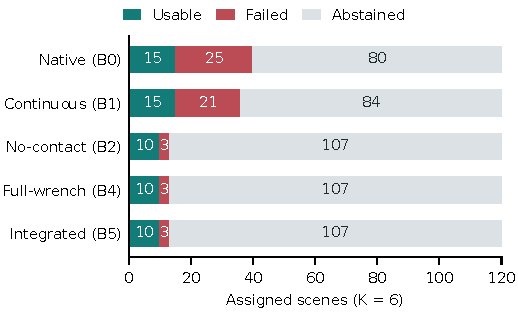
\includegraphics[width=\columnwidth]{selection.pdf}
\caption{K6 choices across all 120 scenes. Every returned candidate in these
rows has a valid future-use outcome, so the middle segment denotes observed
failure, not missing data. B2/B4/B5 choices are identical; B3 and B4-normal
share these aggregate counts. All methods incur the same six-schedule budget.}
\label{fig:selection}
\end{figure}

Native selection returns 40 candidates: 15 usable, 25 failed, 80 abstentions.
Continuous selection returns 36: 15 usable, 21 failed, 84 abstentions
(Fig.~\ref{fig:selection}). Strict B2/B4/B5 selection yields 10 usable,
three failed and 107 abstentions. Conditional usability rises from 15/40
(37.5\%) to 10/13 (76.9\%), but usability per assigned scene falls from
15/120 (12.5\%) to 10/120 (8.3\%). These are descriptive selection consequences,
not a new confirmatory comparison. No utility winner follows without costs
for a failed return and an abstention. Unknown futures elsewhere in the pool
make its oracle a lower bound; the reported regret is not true optimal regret.

\subsection{Historical Model and Library Context}
\label{sec:history}
The earlier V3 study addresses a different intervention: program repair under
compiled primitive physics. On its fresh 360 scenes, K6 native/continuous/
no-contact successes were 128/122/37 for baseline and 141/133/48 for repair.
All 11 no-contact gains were spheres, with no losses; removing the added
topology anchors returned the baseline result. Repair's no-contact counts
were 14, 36 and 48 at $K=1,3,6$. The gain was local to library content and
budget, not broad dexterous grasping competence.

On the same earlier 120 scenes, recompiling the physical model changed
no-contact counts from 18 to 13 for baseline and 24 to 18 for repair. Repair's
native total stayed 43, but seven cases gained and seven lost success. This
changed geometry-dependent bounds and derived quantities as well as inertia;
it was not an isolated inertia intervention. These paired historical results
motivate explicit model and outcome definitions, but are not pooled with V4
or relabeled as its confirmatory monitor benefit. Full tables and the original
V3 uncertainty calculation are in the supplement.

\section{Practical Implications and Limits}
\subsection{Match Evidence to the Intended Claim}
For literal separation, report contact semantics and margins. For absence of
realized non-hand support, report force/torque paths, temporal intervals and
unknowns. For retention after support removal, state the intervention,
snapshot, controls and horizon. For selecting a grasp to use, report usable
returns, failed returns and abstentions with a fixed candidate budget. A
successful historical measurement cannot substitute for the corresponding
future-use test. Nor is a stricter criterion inherently a better predictor.

The evidence supports using the simplest monitor adequate to the declared
target. Here the full-wrench baseline already matches the integrated monitor
on both primary comparisons. The observed geometry and torque redundancy on
controls should not be generalized to all settings: Fetch torque changes
uncertainty, and the fixed controls do not exhaust physically possible cases.
B4/B5 use the same trajectories with no extra physics steps. Their recorded
millisecond scoring times exclude instrumentation, I/O and simulation and do
not establish a runtime advantage.

\subsection{Validity and Access Boundaries}
All evidence is simulated in one engine family, without hardware transfer.
The hand library is finite; the control mechanism mix is constructed, not a
population sample. Source tasks, reference sampling and branch reachability
differ, so aggregate rates do not rank robots. Fixed open-loop removal omits
controller adaptation, other removal mechanisms and longer horizons. Four
DGB identities provide little support for broad object generalization.
The positive control result, retrospective null and fresh selection null are
all needed to avoid turning a diagnostic distinction into a capability claim.

The companion evidence package contains frozen protocols, individual scored
records, sealed choices, future endpoints and offline aggregate reproduction.
A separate core-raw companion supplies the final primitive-control traces;
the full natural-task raw archive is not publicly hosted. Independent raw
adjudication of the complete matrix and clean-machine dynamic reproduction
are not claimed. Third-party dependencies retain their own licensing limits.
The supplement states hashes, exact commands, recovery history, source
versions, data-role boundaries and the limits of each verification level.

\section{Conclusion}
Contact absence, realized load absence and retention after a specified removal
are distinct evaluation targets. Frozen controls demonstrate that the first
can disagree with the second without changing a trajectory, while redundant
support separates loading from intervention-conditioned dependence. Yet the
integrated monitor shows no gain over the full-wrench baseline, rescues no
historical exclusions, and does not improve sealed downstream selection.
The actionable result is to align the claimed property, measurement and
decision cost, and to retain null results and abstentions in the evidence.

\section*{Disclosure}
OpenAI Codex assisted code, analysis tooling and manuscript preparation under
author direction. The author is responsible for all claims; no experiment
isolates an effect of that assistance.
\bibliographystyle{IEEEtran}
\bibliography{references,provenance}
\end{document}
